\part{SW 04 - Data Link Layer - Sicherungsschicht}\label{part:sw04}
\section{Lernziele (Leitfragen)}
\begin{itemize}
    \item Was ist der Unterschied zwischen CSMA/CD und CSMA/CA? Wo werden sie verwendet?
    \item Was ist der Zweck der Sicherungsschicht?
    \item Wie ist die Sicherungsschicht aufgeteilt? Was ist die Hauptaufgabe der LLC und MAC Schichten?
    \item Welches sind die am häufigsten verwendeten Zugriffsverfahren?
    \item Was für Felder findet man in der Sicherungsschicht Frame?
    \item Was sind die wichtigsten Merkmale von MAC Adressen?
    \item Was machen Endgeräte, wenn ihre NIC ein Frame im Medium erkennen?
    \item Wie werden Sicherungsschicht Frames in einem Switch bearbeitet?
    \item Wie funktioniert der \flqq Learn-and-forward\frqq{} Prozess?
    \item Was ist der Unterschied zwischen \flqq Unicast\frqq{} und \flqq Broadcast\frqq{} Frames?
    \item Was ist der Zweck ARPs?
    \item Wie funktioniert ARP?
\end{itemize}

\section{Antworten}
\subsection*{Was ist der Unterschied zwischen CSMA/CD und CSMA/CA? Wo werden sie verwendet?}\label{sub:csma}\index{CSMA - Carrier Sense Multiple Access}
//TODO Sollte für die Logik zu SW03 T1 verschoben werden.\\

\textbf{CSMA: Carrier Sense Multiple Access}
\begin{itemize}
    \item Sender hört den Datenverkehr auf der Leitung ab (= carrier sense)
    \item Sender wartet, bis der Kanal frei ist
    \item sobald der Kanal frei ist, darf gesendet werden
    \item falls mehrere Sender (fast) gleichzeitig anfangen zu senden:\\Kollision $\rightarrow$ Wiederholung nach zufälliger Zeitspanne
\end{itemize}\,\\

\textbf{CSMA/CA (CA = Collision Avoidance)}
\begin{itemize}
    \item Kollisionsvermeidung durch zufällige Wartezeit nach Erkennung eines freien Kanals
    \item z.B. WLAN 802.11-DCF (Distributed Coordination Function)
\end{itemize}\,\\

\textbf{CSMA/CD (Collision Detection)}
\begin{itemize}
    \item sobald eine Kollision erkannt wird, wird die Übertragung abgebrochen
    \item z.B. Ethernet
\end{itemize}\,\\

\begin{tabularx}{\textwidth}{X|X}
    \multicolumn{1}{X}{CSMA/CD}&\multicolumn{1}{X}{CSMA/CA}\\
    \hline
    $\bullet$ Greift nach der Kollision&$\bullet$ Greift vor der Kollision\\
    $\bullet$ Genutzt in kabelgebundenen Netzwerken&$\bullet$ Genutzt in kabellosen Netzwerken\\
    $\bullet$ Reduziert die `'recovery time'' nach einer Kollision&$\bullet$ Minimiert Kollisionsgefahr\\
    $\bullet$ Bei Konflikt wird erneut gesendet&$\bullet$ Sendet zuerst die Info, dass etwas übermittelt wird\\
    $\bullet$ Effektiver als das einfache CSMA&$\bullet$ ähnlich effizient wie CSMA\\
\end{tabularx}


\subsection*{Was ist der Zweck der Sicherungsschicht?}\label{sub:Sicherungsschicht}
\begin{itemize}
    \item Kommunikation zwischen Netzwerkkarten der Endgeräten
    \item ermöglicht höheren Protokollen den Zugriff auf die Physikalische Schicht 1
    \item Kapselt Pakete (IPv4 und IPv6) in das Layer 2 Frame
    \item Fehlererkennung und Abweisen von korrumpierten Frames
\end{itemize}
Siehe auch \underline{\hyperref[sub:SchichtenOSIModell]{Schichten des OSI Modells}} (Seite \pageref{sub:SchichtenOSIModell}).

\pagebreak
\subsection*{Wie ist die Sicherungsschicht aufgeteilt? Was ist die Hauptaufgabe der LLC und MAC Schichten?}\label{sub:LLC_MAC}\index{LLC - Logical Link Control}\index{MAC - Media Access Control}
\begin{itemize}
    \item Logical Link Control (LLC) kommuniziert zwischen Netzwerksoftware der oberen Schichten und der MAC-Subschicht.
    \item Media Access Control (MAC) ist für die Datenkapselung und Verwaltung des Zugriffs auf das Übertragungsmedium verantwortlich. Siehe Frage oben \underline{\hyperref[sub:csma]{Unterschied CSMA/CD und CSMA/CA}}, Seite \pageref{sub:csma}.
\end{itemize}

\begin{figure}[H]
    \begin{center}
    \label{pic:DataLinkLayer_LLC_MAC}
    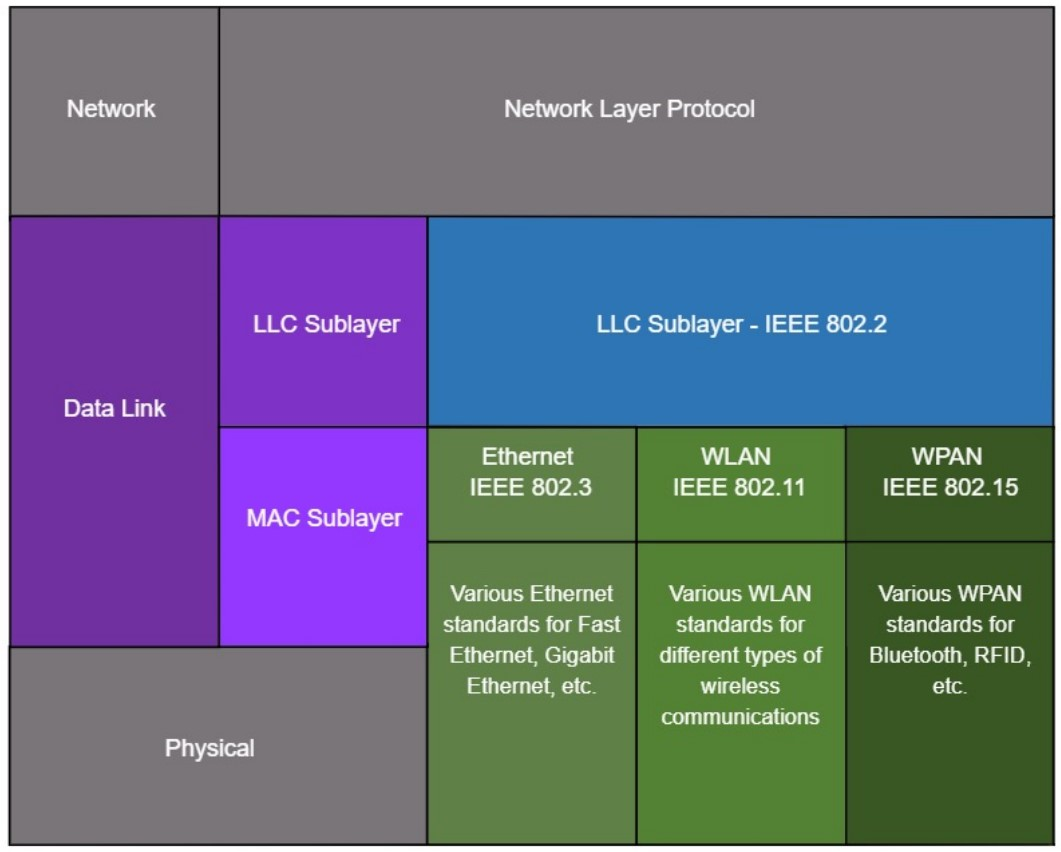
\includegraphics[width=\textwidth]{images/DLL_Sublayers.jpg}
    \caption{Subschichten der Sicherungsschicht / des Data Link Layers (\textsuperscript{\textcopyright}Cisco)}
    \end{center}
\end{figure}

\subsection*{Welches sind die am häufigsten verwendeten Zugriffsverfahren?}
//TODO

\subsection*{Was für Felder findet man in der Sicherungsschicht Frame?}
Es gibt einen \textbf{Header}, \textbf{Data} und einen \textbf{Trailer}. Header und Trailer sind einzelne Felder unterteilt:

\begin{figure}[H]
    \begin{center}
    \label{pic:DataLinkFrame}
    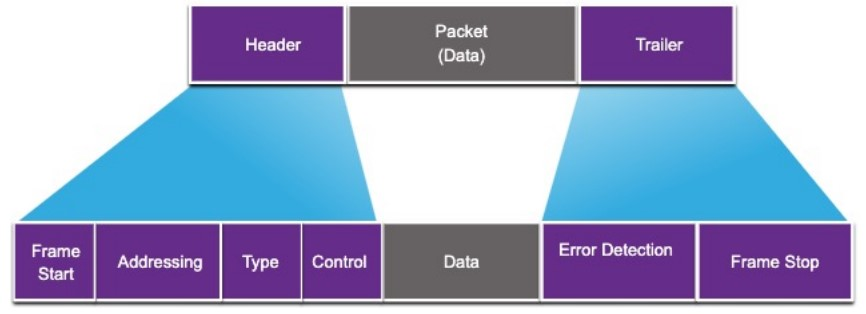
\includegraphics[width=\textwidth]{images/Data_Link_Frame.jpg}
    \caption{Aufbau eines Data Link Frames (\textsuperscript{\textcopyright}Cisco)}
    \end{center}
\end{figure}

\begin{tabularx}{\textwidth}{lX}
    Feld&Beschreibung\\
    \hline
    Frame Start / Stop&Identifiziert den Anfang und das Ende des Frames\\
    Addressing&Zeigt Source und Destination Knoten (nodes) an\\
    Type&Identifiziert gekapseltes Protokoll von Layer 3\\
    Control&Identifiziert Dienste für die Flusskontrolle\\
    Data&Enthält die "`Zuladung"' (payload), die zu übermittelnden Daten\\
    Error Detection&Wird verwendet um Übermittlungsfehler zu entdecken\\
    \hline
\end{tabularx}\\

Das "`Addressing"'-Feld besteht aus zwei Einträgen, nämlich die MAC-Adressen der Netzwerkkarten\\
(Siehe Glossar: \acrshort{nic})\index{NIC - \acrlong{nic}} vom Ursprung und vom Ziel (Source, Destination). Diese wird an jedem Knoten (node) geändert.

\begin{figure}[H]
    \begin{center}
    \label{pic:DataLinkFrameAddresses}
    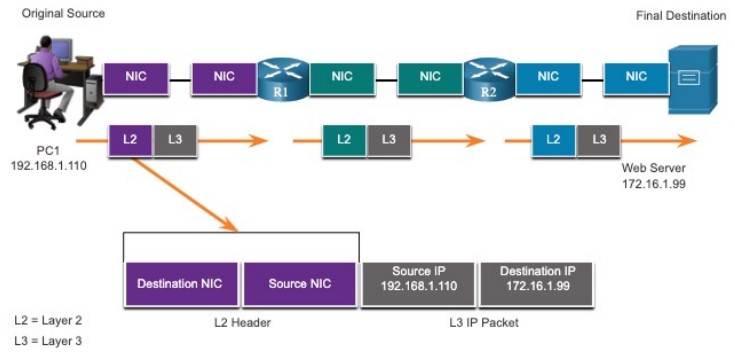
\includegraphics[width=\textwidth]{images/Data_Link_Frame_Addresses.jpg}
    \caption{MAC-Adressen werden an jedem Knotenpunkt geändert. (\textsuperscript{\textcopyright}Cisco)}
    \end{center}
\end{figure}

\subsection*{Was sind die wichtigsten Merkmale von MAC Adressen?}\index{MAC!Adresse}
\begin{itemize}
    \item 48 bits = 12 hex-Ziffern = 6 bytes
    \item einzigartig
    \item Erste Hälfte von Hersteller, zweite Hälfte zufällig
\end{itemize}
Beispiel Darstellung einer MAC-Adresse: 3D-8F-45-27-3C-1A oder 3D:8F:45:27:3C:1A

\subsection*{Was machen Endgeräte, wenn ihre NIC ein Frame im Medium erkennen?}\label{sub:Frameerkennung}\index{NIC - \acrlong{nic}}\index{Unicast}\index{Broadcast}\index{MAC!Adresse}
\begin{enumerate}
    \item Untersucht die Ziel MAC-Adresse
    \item Stimmt MAC-Adresse mit der eigenen überein (oder Broadcast/Multicast)?
    \begin{itemize}
        \item Keine Übereinstimmung: \textbf{ignoriere} (ignore) den Frame
        \item Übereinstimmung: \textbf{verarbeite} (process) und übergebe Frame den höheren Schichten
    \end{itemize}
\end{enumerate}

\begin{figure}[H]
    \begin{center}
    \label{pic:EthernetFrameProcessing}
    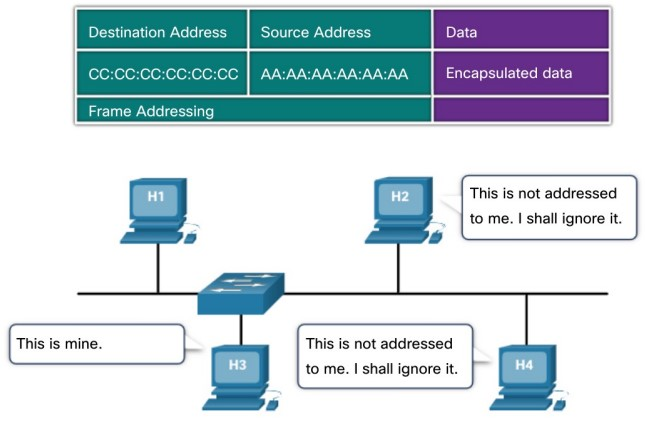
\includegraphics[width=\textwidth]{images/Frame_processing.jpg}
    \caption{Verhalten der Netzwerkkarten (\textsuperscript{\textcopyright}Cisco)}
    \end{center}
\end{figure}

\subsection*{Wie werden Sicherungsschicht Frames in einem Switch bearbeitet? }\index{Switch}\index{MAC!Adresse}
Ethernet-Switches
\begin{itemize}
    \item \dots{}nutzen MAC-Adressen, um Weiterleitungsentscheidungen (forwarding decision) zu treffen
    \item \dots{}sind unwissend über den Inhalt der Daten im Datenfeld
    \item \dots{}Entscheidungen über die Weiterleitung beruhen lediglich auf die Ethernet MAC-Adressen vom Layer 2
    \item \dots{}untersuchen eigene MAC-Adressentabellen um Entscheidungen für jedes Frame zu treffen
    \item Wenn ein Switch einschaltet, ist seine MAC-Adresstabelle leer
\end{itemize}


\subsection*{Wie funktioniert der \flqq Learn-and-forward\frqq{} Prozess?}\index{Switch!Learn and Forward}\index{MAC!Adresse}
I. LEARN: Untersuche die Source-MAC-Adresse
\begin{enumerate}
    \item Ein Frame erreicht den Switch
    \item Switch untersucht die Source-MAC-Adresse des Frames und die Port-Nummer des Einganges
    \item Source-MAC-Adresse nicht in Tabelle vorhanden:
    \begin{itemize}
        \item[$\rightarrow$] füge Source-MAC-Adresse und Port-Nummer des Einganges zur MAC-Adresstabelle
    \end{itemize}
    \item[3.] Source-MAC-Adresse in Tabelle vorhanden:
    \begin{itemize}
        \item[$\rightarrow$] Erneuere den Timer für den Eintrag in der Tabelle. Standard 5 min
    \end{itemize}
    \item[3.] Source-MAC-Adresse vorhanden, aber anderer Port:
    \begin{itemize}
        \item[$\rightarrow$] ersetze Port und Timer-Update
    \end{itemize}
\end{enumerate}\,\\[1em]

\newpage
II. FORWARD: Finde Destination-MAC-Adresse
\begin{itemize}
    \item Destination-MAC-Adresse ist unicast:
    \begin{itemize}
        \item Finde Übereinstimmung der Destination-MAC-Adresse in der Tabelle
        \begin{itemize}
            \item Eintrag gefunden $\rightarrow$ weiterleiten des Frames an der in der Tabelle \textbf{eingetragenen} Port
            \item keinen Eintrag gefunden $\rightarrow$ weiterleiten des Frames an \textbf{alle} Port, \textbf{ausser Eingangsport}
        \end{itemize}
    \end{itemize}
\end{itemize}

\subsection*{Was ist der Unterschied zwischen \flqq Unicast\frqq{} und \flqq Broadcast\frqq{} Frames?}\index{Unicast}\index{Broadcast}\index{MAC!Adresse}
Unicast-Frames haben die MAC-Adresse ein spezifischen Zieles angegeben,

\subsection*{Was ist der Zweck ARPs?}\index{ARP - Address Resolution Protocol}\index{MAC!Adresse}
Das Address Resolution Protocol vermittelt zwischen der Sicherungsschicht - Data Link (2) und der Vermittlungsschicht - Network (3). Es dient dazu, zu einer bekannten Netzwerkadresse der Internetschicht (IPv4-Adresse) die physische Adresse der Sicherungsschicht (MAC-Adresse) zu ermitteln. Die ermittelte MAC-Adresse wird in einer ARP-Tabelle hinterlegt.

\subsection*{Wie funktioniert ARP?}\index{ARP - Address Resolution Protocol}\index{MAC!Adresse}
Angenommen die ARP-Tabelle ist leer. Meine NIC\index{NIC - \acrlong{nic}} möchte die MAC-Adresse vom Standardgateway wissen. Zunächst wird ein \textbf{ARP request} gesendet mit Destination "`FF-FF-FF-FF-FF-FF"', also ein Broadcast. Alle Geräte erhalten den Aufruf und entscheiden (Siehe \underline{\hyperref[sub:Frameerkennung]{Frame-Erkennung}}, Seite \pageref{sub:Frameerkennung}). Der Gateway antwortet daraufhin mit einem \textbf{ARP reply} und teilt meiner NIC seine MAC-Adresse mit. Diese wird in die eigene ARP-Tabelle eingetragen.